
%%%%%%%%%%%%%%%%%%%% author.tex %%%%%%%%%%%%%%%%%%%%%%%%%%%%%%%%%%%
%
% sample root file for your "contribution" to a proceedings volume
%
% Use this file as a template for your own input.
%
%%%%%%%%%%%%%%%% Springer %%%%%%%%%%%%%%%%%%%%%%%%%%%%%%%%%%


\documentclass{svproc}
%
% RECOMMENDED %%%%%%%%%%%%%%%%%%%%%%%%%%%%%%%%%%%%%%%%%%%%%%%%%%%
%
\usepackage{graphicx}
\usepackage{hyperref}
\usepackage{amsmath}% http://ctan.org/pkg/amsmath
\newcommand{\thickhat}[1]{\mathbf{\hat{\text{$#1$}}}}
\newcommand{\thickbar}[1]{\mathbf{\bar{\text{$#1$}}}}
\newcommand{\thicktilde}[1]{\mathbf{\tilde{\text{$#1$}}}}
\usepackage{subfig}
\usepackage{cite}
\usepackage{amsmath}
\usepackage{multicol}
\usepackage{array}
\usepackage{float}
\usepackage{subfig}
\newcolumntype{x}[1]{>{\centering\arraybackslash\hspace{0pt}}p{#1}}

% to typeset URLs, URIs, and DOIs
\usepackage{url}
\def\UrlFont{\rmfamily}


%\usepackage[english,spanish]{babel}
%\AtBeginDocument{\selectlanguage{spanish}}
%\renewcommand{\figurename}{Figura}
%\renewcommand{\refname}{Referencias}
%\renewcommand{\tablename}{Tabla}

\begin{document}
\mainmatter              % start of a contribution
%
\title{Analysis of SplitThreader: A web tool for exploration and analysis of rearrangements in cancer genomes}
%
\titlerunning{Analysis of SplitThreader}  

\author{Vicente Machaca Arceda }
\authorrunning{Vicente Machaca Arceda et al.} 
\tocauthor{Vicente Machaca Arceda}
\institute{Universidad Nacional de San Agustín, Arequipa-Perú,\\
\email{vmachacaa@unsa.edu.pe}} 


\maketitle             

\begin{abstract}

In this work, we reviewed and replicated the results of SplitThreader. It is a web tool for the analysis of structural variants in cancer genomes. This tool uses a variant calling file with a profile of copy numbers in order to graphically show copy number variants and gene fusions. Moreover, the proposal, represents structural variants in a graph, then it uses a priority queue breath-first search to detect gene fusions. Furthermore, SplitThreader is open source and it is easy to use, its architecture is based on PHP, Javascript, R and Python. Finally, SplitThreader is a usefull tool that helps the analysis of structural variants, nevertheless it depends on other tools/algorithms like Lumpy and Sniffles that limit its performance.

\keywords{SplitThreader, cancer genomcs, visualization }
\end{abstract}


%- Introducción: Contexto, Problema, Objetivo o Pregunta de Principal que el
%proyecto pretende dar respuesta.
%- Data Set: Presentación del conjunto de datos con alguna visualización de los
%mismos. Informar cualquier dificultad o problema asociado con el conjunto de
%datos, incluidos los análisis fallidos.
%- Marco Teórico: Breve descripción de los métodos utilizados para el proyecto y
%sus fundamentos.
%- Trabajos Relacionados: Principales trabajos relevantes que intentan resolver
%el problema planteado

%- Propuesta: Presentación de cómo se ha realizado el análisis real. Descripción
%de la arquitectura o flujo de información (pipeline) de la propuesta de solución al
%problema planteado. Incluir los algoritmos, programas o paquetes y su
%utilización.
%- Evaluación: Presentación de los resultados y su interpretación - gráficos muy
%recomendable.
%- Conclusiones: Conclusiones finales del estudio, tanto de fracasos como
%aciertos. En caso de falla, debería ser discutido los motivos y recomendaciones
%para el futuro que ayudarían a evitar los problemas encontrados.

%%%%%%%%%%%%%%%%%%%%%%%%%%%%%%%%%%%%%%%%%%%%%%%%%%%%%%%%%%%%%%%%%%%%%%%%%%%%%%%%%%%%%
%%%%%%%%%%%%%%%%%%%%%%%%%%%%%%%%%%%%%%%%%%%%%%%%%%%%%%%%%%%%%%%%%%%%%%%%%%%%%%%%%%%%%
\section{Introduction} 
%%%%%%%%%%%%%%%%%%%%%%%%%%%%%%%%%%%%%%%%%%%%%%%%%%%%%%%%%%%%%%%%%%%%%%%%%%%%%%%%%%%%%
%%%%%%%%%%%%%%%%%%%%%%%%%%%%%%%%%%%%%%%%%%%%%%%%%%%%%%%%%%%%%%%%%%%%%%%%%%%%%%%%%%%%%

Genomics data has growth up exponentially, for example in 2009, they reached about 0.8 ZB, moreover in 2020 they reached about 40 ZB \cite{prabahar2016perspectives}. Furthermore, cancer related data are generated from: gene expression data (Microarray), NGS data, protein–protein interaction (PPI), pathway annotation data y gene ontology (GO). These data are important for research in cancer diagnosis and treatment. Big data resources allow researchers to observe large retrospective, and heterogeneous data of cancer patients \cite{berman2013principles}.\\

For instance, the human genome is made of approximately 3.2 billions bp of DNA \cite{archibald2018genomics}. The HIV-1 genome is made of 20k bp of DNA, meanwhile the COVID-19 is made of 32k bp \cite{randhawa2020machine}. Additionally, there are approximately 19000 to 25000 genes (no one knows for sure) \cite{archibald2018genomics}. Finally, human genes have dozens of introns, each of which can be tens of thousands of nucleotides. Distinguishing exons from introns and other forms of non-coding DNA is challenging \cite{archibald2018genomics}. This lack of information, makes difficult the research in cancer genomics.\\

Moreover, genomic instability is one of the hallmarks of cancer \cite{hanahan2011hallmarks,hastings2009mechanisms},	resulting in a widespread copy number changes, structural variants and chromosome-scale rearrangements \cite{nattestad2016splitthreader}. Furthermore, copy number variants and gene fusions are common drivers in cancer \cite{shlien2009copy, mitelman2007impact}. In this context, it is very important to detect these structural variants, but the available algorithms for identifying gene fusions do not have perfect specificity (false positive rate)  and they require a joint analysis of genomic and transcriptomic data. Moreover, rearrangements variants are difficult to study because of the sheer complexity of rearrangements, which often include adjacencies between distant regions of a chromosome or even between unrelated chromosomes \cite{nattestad2016splitthreader}.  \\

In this work, we reviewed and replicated the tool SplitThreader \cite{nattestad2016splitthreader}. It is an open source interactive web application for analysis and visualization of genomics rearrangements and copy number variation in cancer genomes. \\


%%%%%%%%%%%%%%%%%%%%%%%%%%%%%%%%%%%%%%%%%%%%%%%%%%%%%%%%%%%%%%%%%%%%%%%%%%%%%%%%%%%%%
%%%%%%%%%%%%%%%%%%%%%%%%%%%%%%%%%%%%%%%%%%%%%%%%%%%%%%%%%%%%%%%%%%%%%%%%%%%%%%%%%%%%%
%\section{Data} 
%%%%%%%%%%%%%%%%%%%%%%%%%%%%%%%%%%%%%%%%%%%%%%%%%%%%%%%%%%%%%%%%%%%%%%%%%%%%%%%%%%%%%
%%%%%%%%%%%%%%%%%%%%%%%%%%%%%%%%%%%%%%%%%%%%%%%%%%%%%%%%%%%%%%%%%%%%%%%%%%%%%%%%%%%%%


%%%%%%%%%%%%%%%%%%%%%%%%%%%%%%%%%%%%%%%%%%%%%%%%%%%%%%%%%%%%%%%%%%%%%%%%%%%%%%%%%%%%%
%%%%%%%%%%%%%%%%%%%%%%%%%%%%%%%%%%%%%%%%%%%%%%%%%%%%%%%%%%%%%%%%%%%%%%%%%%%%%%%%%%%%%
\section{Concepts} 
%%%%%%%%%%%%%%%%%%%%%%%%%%%%%%%%%%%%%%%%%%%%%%%%%%%%%%%%%%%%%%%%%%%%%%%%%%%%%%%%%%%%%
%%%%%%%%%%%%%%%%%%%%%%%%%%%%%%%%%%%%%%%%%%%%%%%%%%%%%%%%%%%%%%%%%%%%%%%%%%%%%%%%%%%%%

In this section, we present the most relevant concepts related to bioinformatics and cancer genomics.

\subsection{Genomics data}

``DNA is abbreviation of deoxyribonucleic acid, organic chemical of complex molecular structure that is found in all prokaryotic and eukaryotic cells and in many viruses. DNA codes genetic information for the transmission of inherited traits'' \cite{dna_definition}. Moreover, the term genomics is used to refer the sum total of DNA in cells \cite{archibald2018genomics}. For instance, in Figure \ref{fig:dna}, we present a piece of COVID-19 DNA (genome) in FASTA format. DNA data is just a string of four characters: A, C, G, T that represent the nitrogen bases Adenine, Cytosine, Guanine and Thymine respectively. Unfortunately, this data is not 100\% accurate and for a single human genome, it could reaches about 4 GB (3.2 billion bases).    


\begin{figure}[H]
	\centering
	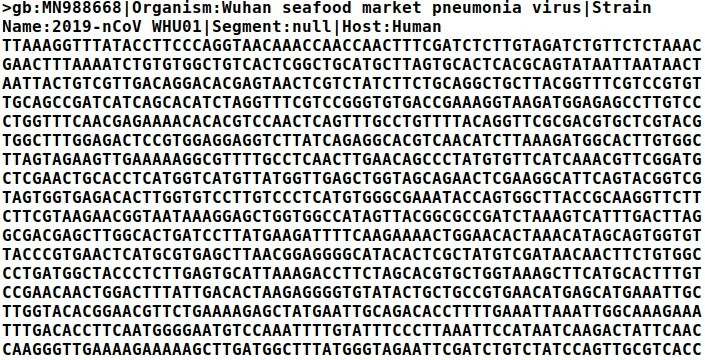
\includegraphics[width=0.6\textwidth]{img/splitthreader/dna}
	\caption{A piece of COVID-19 DNA.}
	\label{fig:dna}
\end{figure}

\subsection{Sequence alignment}
In Bio-informatics, sequence alignment could be defined as a way to arranging DNA, RNA and amino-acids  sequences in order to find similarities \cite{xiong2006essential}. For example, in Figure \ref{fig:al1}, we present two alignments, the top alignment (no alignment) seems to denote that there is not identity or similarity regions between two sequences, meanwhile, the bottom alignment shows that both sequences are similar.


\begin{figure}[h]
	\centering
	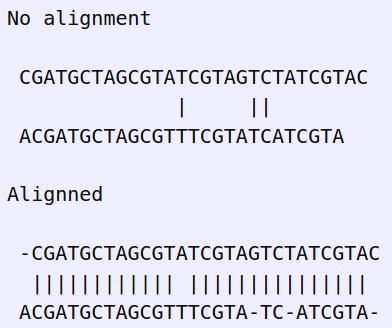
\includegraphics[width=0.3\textwidth]{img/splitthreader/al1}
	\caption{Example of sequence alignment adding gaps.}
	\label{fig:al1}
\end{figure}

\subsubsection{Concordance reads}
.- This type of alignment refers when the reads have span size within the range of expected fragment size and consistent orientation of read pairs with respect to reference \cite{alig_2021}.

\subsubsection{Discordance reads}
.- In this case, the reads have unexpected span size or inconsistent orientation of read pairs. It is important to identify this type of read in order to analyze genome alteration events \cite{alig_2021}.

\subsubsection{Split reads}
.- When one portion of an read, maps to several locations of the same read map. Then, these are reads that have two or more alignments to the reference from unique region of the read. \cite{alig_2021}.

\subsection{Structural variants}
According to the National Center for Biotechnology Information (NCBI): ``Structural variation (SV) is generally defined as a region of DNA approximately 1 kb and larger in size and can include inversions and balanced translocations or genomic imbalances (insertions and deletions), commonly referred to as copy number variants (CNVs)'' \cite{sv_ncbi_2021}. In other words, this variations represent mutation in DNA, this mutations could be: insertions, deletions, inversions and translocations. In Figure \ref{fig:variants}, we present some examples.


\begin{figure}[h]
	\centering
	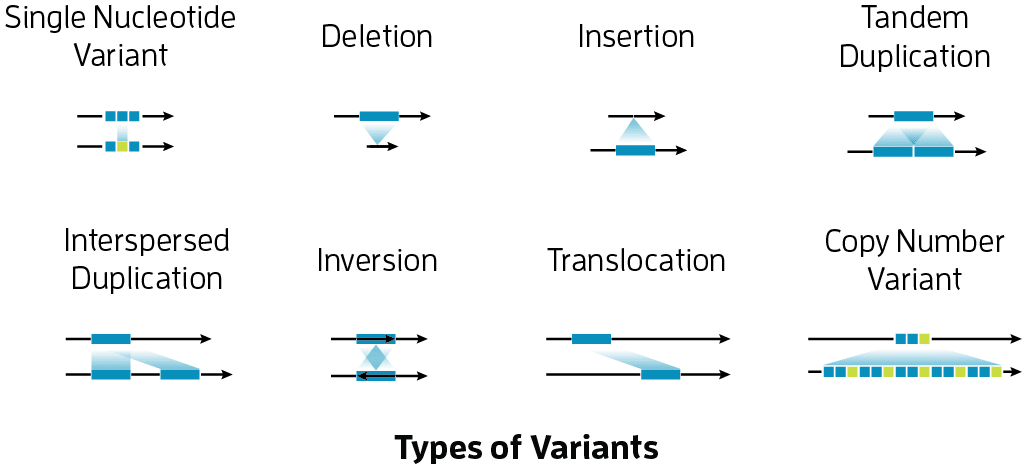
\includegraphics[width=0.7\textwidth]{img/splitthreader/variants}
	\caption{Example of structural variants. Source: \cite{sv_pacbio_2021}}
	\label{fig:variants}
\end{figure}

\subsubsection{Copy number variants}

.- According to the National Human Genome (NIH): ``A copy number variation (CNV) is when the number of copies of a particular gene varies from one individual to the next'' \cite{cnv_nih_2021}. For example in Figure \ref{fig:cnv}, we present some examples of CNV, we could see how the number of genes varies individual 2 to 6. Additionally, it is recognized that some cancer diseases are associated to CNV \cite{cnv_nih_2021, nattestad2016splitthreader, shlien2009copy, mitelman2007impact}.

\begin{figure}[h]
	\centering
	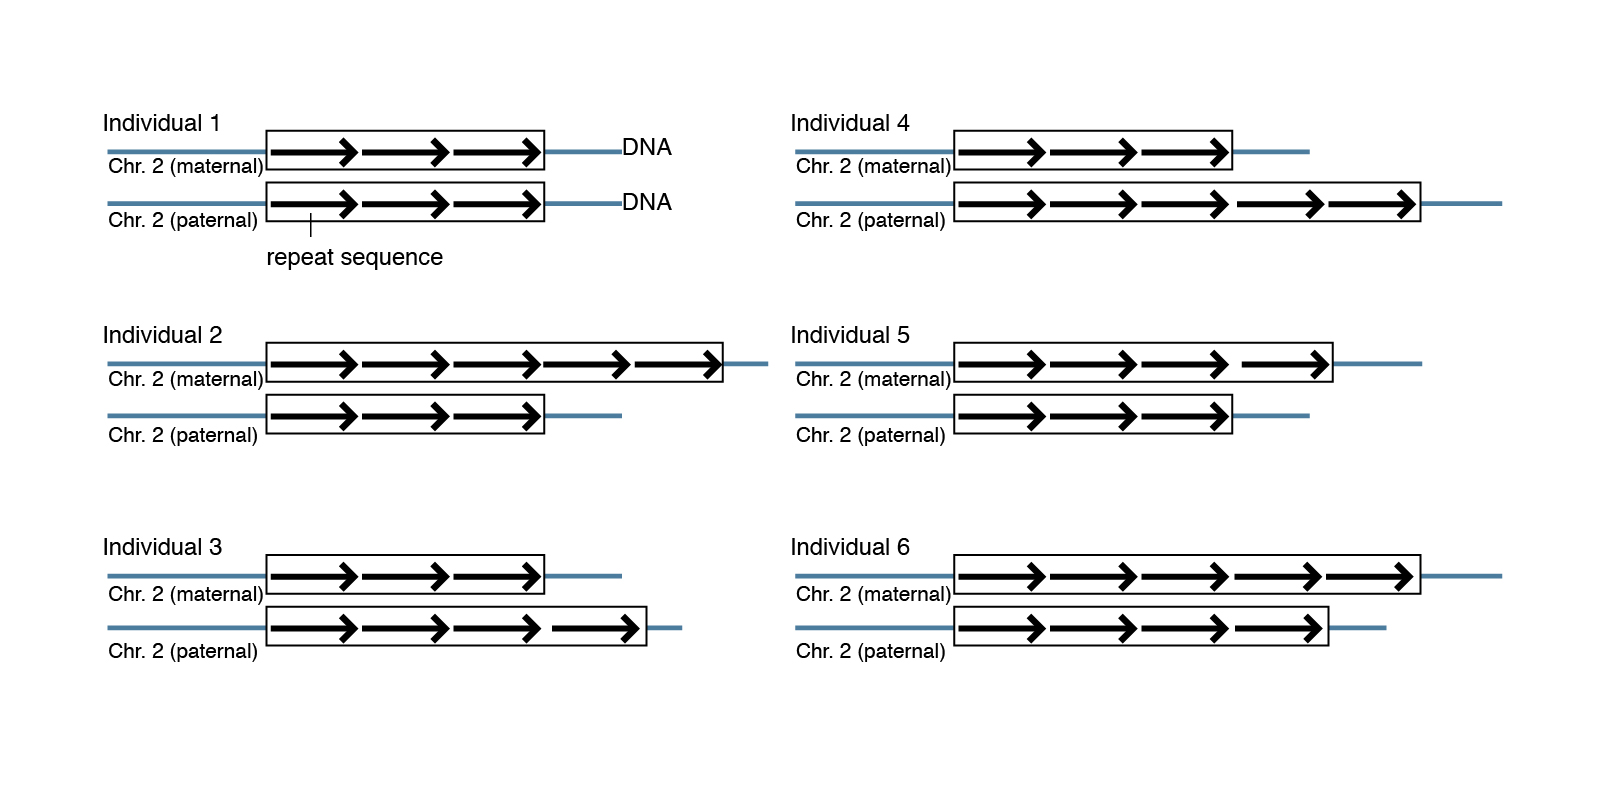
\includegraphics[width=0.8\textwidth]{img/splitthreader/copy_number_variation}
	\caption{Example of copy number variation. Source: \cite{cnv_nih_2021}}
	\label{fig:cnv}
\end{figure}



\subsubsection{Gene fusions}

.- Gene fusion is a gene made by two or more genes \cite{genefusion_nih_2021}. For example, the first gene
fusion discovered in cancer was BCR/ABL (related to leukemia), it is resulted from a fusion of chromosomes \cite{stam1985evidence}.

%%%%%%%%%%%%%%%%%%%%%%%%%%%%%%%%%%%%%%%%%%%%%%%%%%%%%%%%%%%%%%%%%%%%%%%%%%%%%%%%%%%%%
%%%%%%%%%%%%%%%%%%%%%%%%%%%%%%%%%%%%%%%%%%%%%%%%%%%%%%%%%%%%%%%%%%%%%%%%%%%%%%%%%%%%%
\section{Related work} 
%%%%%%%%%%%%%%%%%%%%%%%%%%%%%%%%%%%%%%%%%%%%%%%%%%%%%%%%%%%%%%%%%%%%%%%%%%%%%%%%%%%%%
%%%%%%%%%%%%%%%%%%%%%%%%%%%%%%%%%%%%%%%%%%%%%%%%%%%%%%%%%%%%%%%%%%%%%%%%%%%%%%%%%%%%%

Detection of structural variants are the key point in cancer rearrangement analysis. For example, Lumpy \cite{layer2014lumpy}, stands as a probabilistic framework for structural variant discovery. This framework uses three alignments inputs: concordant alignment, discordant alignment and split reads. Then, it uses a probabilistic method to detect structural variants like breakpoints (a pair of bases that are adjacent in an sequence sampĺe but not in the reference genome). \\

Furthermore, there are studies about the perspective and challenges of structural variant detection for precision oncology \cite{van2021structural}. Some techniques are used for short-reads \cite{ruffalo2011comparative, liu2015structural}. For long-read sequencing, technologies like PacBio and Oxford Nanopore Technologies (ONT) are valuable for structural variant detection \cite{de2019newest}. Moreover, some algorithms have been develop to improve the quality of alignments and structural variant detection \cite{rang2018squiggle, travers2010flexible}.\\

Despite, there are many techniques to detect structural variants, they does not have 100\% accuracy. Furthermore, it is difficult to evaluate and see the structural variants from Variant Call Files (VCF), these are files that represent the structural variants detected in genomes. In this context, there are some visualization tools, that stand for the analysis and discovery of structural variants. SplitThreader \cite{nattestad2016splitthreader}, for example, is used to graphically see copy number variations. Additionally, this tool used an algorithm to detect gene fusions.\\

MoMI-G is other tool that used a graph-based approach to represent structural variants \cite{yokoyama2019momi}. This tool, used the same methodology of SplitThreader, but it is designed specifically for long-reads. Finally, there are several tools to detect and analyze structural variants,  some authors reviewed and analyzed them \cite{yokoyama2020visualization}.

%%%%%%%%%%%%%%%%%%%%%%%%%%%%%%%%%%%%%%%%%%%%%%%%%%%%%%%%%%%%%%%%%%%%%%%%%%%%%%%%%%%%%
%%%%%%%%%%%%%%%%%%%%%%%%%%%%%%%%%%%%%%%%%%%%%%%%%%%%%%%%%%%%%%%%%%%%%%%%%%%%%%%%%%%%%
\section{Proposal} 
%%%%%%%%%%%%%%%%%%%%%%%%%%%%%%%%%%%%%%%%%%%%%%%%%%%%%%%%%%%%%%%%%%%%%%%%%%%%%%%%%%%%%
%%%%%%%%%%%%%%%%%%%%%%%%%%%%%%%%%%%%%%%%%%%%%%%%%%%%%%%%%%%%%%%%%%%%%%%%%%%%%%%%%%%%%

In this work, we replicated the results of SplitThreader \cite{nattestad2016splitthreader}. This is a open source web application that stand for  analysis and visualization of genomic rearrangements and copy number variation in cancer genomes. It constructs a graph of genomic rearrangements and uses a priority queue breadth-first search algorithm to search for novel interactions.\\

SplitThreader follows the pipeline in Figure \ref{fig:pipeline}. First, we aligns the sample genome with a reference genome using SpeedSeq (we could use another tool that generated bam files). After alignment, three files are generated: concordance alignment, discordance alignment and split-reads. These files are taken by Lumpy and Copycat in order to detect structural variants. This step, generates two files: a variant calling file and a copy number file, these files are taken by SplitThreader in order to detect gene fusions, then SplitThreader plot the rearrangements using circle plots. \\

\begin{figure}[h]
	\centering
	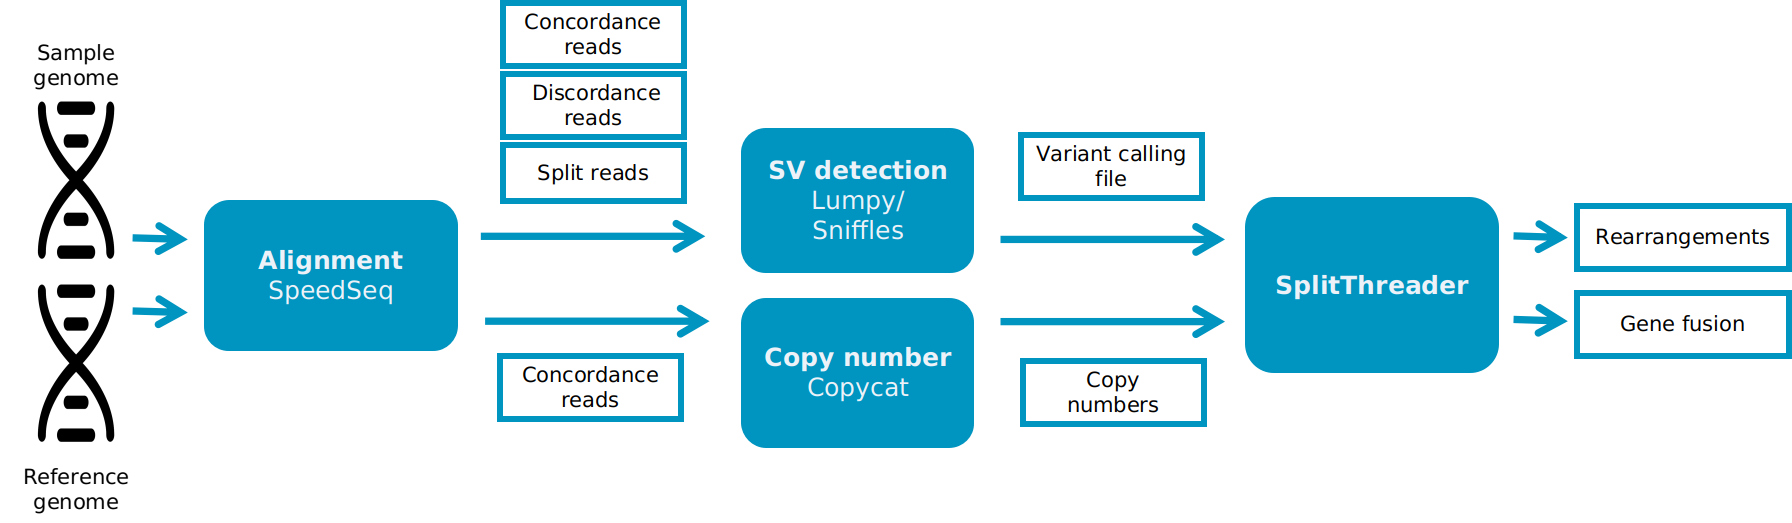
\includegraphics[width=\textwidth]{img/splitthreader/pipeline}
	\caption{SplitThreader pipeline. Two sequences are aligned using SpeedSeq, then output files are taken by Lumpy and Copycat in order to detect structural variants, finally SplitThreader takes its outputs and plot the rearrangements and gene fusions.}
	\label{fig:pipeline}
\end{figure}


Formally, SplitThreader uses a graph, where a node represent sequences from DNA (reference genome) spanning between rearrangements breakpoints. Moreover, edges are used to represent rearrangements variants and no-rearranged reference-spanning connections. First, the graph is constructed where each node represents a chromosome, then each node is split each time we detect breakpoints. In Figure \ref{fig:graph}, we present this graph-based approach. \\

\begin{figure}[h]
	\centering
	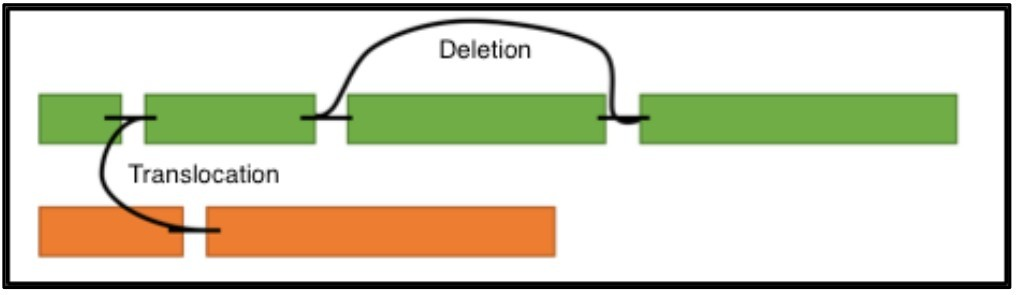
\includegraphics[width=0.6\textwidth]{img/splitthreader/graph}
	\caption{Representation of rearrangements using a graph-based approach (SplitThreader proposal). Source: \cite{nattestad2016splitthreader}}
	\label{fig:graph}
\end{figure}



\subsection{Gene fusion detection}
Normally, gene fusion could be detected using RNA-seq and PCR validation to confirm transcriptome link between fusion genes \cite{edgren2011identification}. However, there are scenarios where this analysis could no detect all gene fusions. For instance, when there is not a single variant that intersect both gene, when cancer genomes have ``two hop'' gene fusions and when the corresponding genomic region are not directly fused to each other but instead, it require passing through a third or more genomic region. \\

SplitThreader detect gene fusions searching for the shortest and lowest variant count path that connects the fusion genes. SplitThread uses a priority queue breath-first search to detect the shortest path in base pairs connecting two genes.\\

\subsection{Variant neighborhood and copy number concordance}
SplitThreader, can detect rearrangements responsible for copy number changes. The Web tool, categorizes each rearrangement variant by its copy number concordance. These concordances could be: matching, partial, non-matching or neutral. Finally, SplitThreader categorize each the rearrangements like reciprocal, simple, solo or crowded. 

\begin{figure}[h]
	\centering
	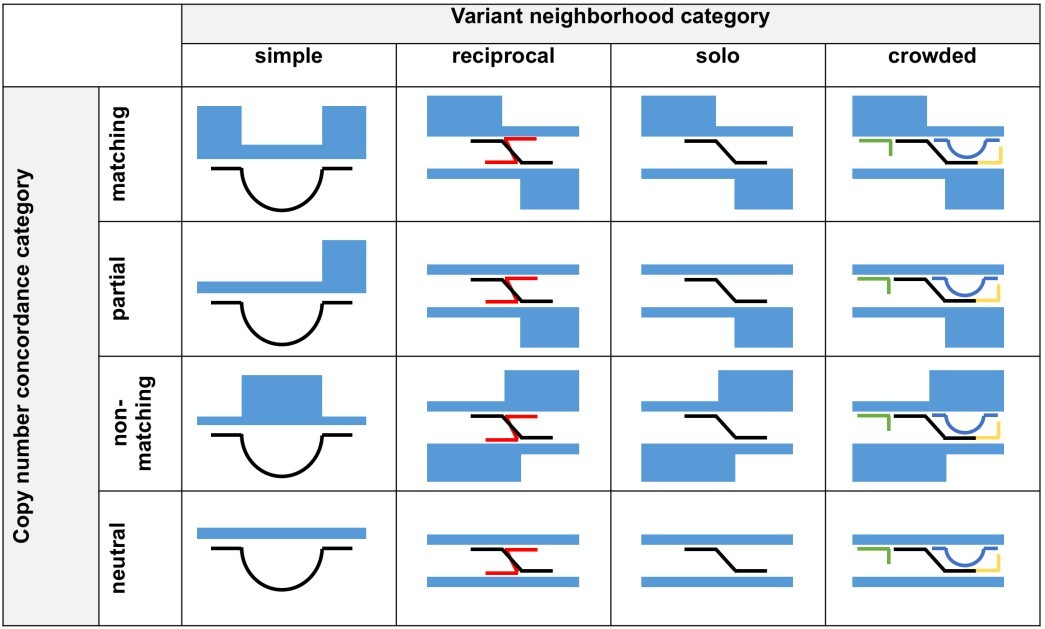
\includegraphics[width=0.8\textwidth]{img/splitthreader/var_cat}
	\caption{Variant rearrangement categorization propose by SplitThreader based on copy number concordance. Source: \cite{nattestad2016splitthreader}}
	\label{fig:graph}
\end{figure}

%%%%%%%%%%%%%%%%%%%%%%%%%%%%%%%%%%%%%%%%%%%%%%%%%%%%%%%%%%%%%%%%%%%%%%%%%%%%%%%%%%%%%
%%%%%%%%%%%%%%%%%%%%%%%%%%%%%%%%%%%%%%%%%%%%%%%%%%%%%%%%%%%%%%%%%%%%%%%%%%%%%%%%%%%%%
\section{Results} 
%%%%%%%%%%%%%%%%%%%%%%%%%%%%%%%%%%%%%%%%%%%%%%%%%%%%%%%%%%%%%%%%%%%%%%%%%%%%%%%%%%%%%
%%%%%%%%%%%%%%%%%%%%%%%%%%%%%%%%%%%%%%%%%%%%%%%%%%%%%%%%%%%%%%%%%%%%%%%%%%%%%%%%%%%%%

In this work we deployed SplitThreader locally. This Web tool is hosted on \href{https://github.com/MariaNattestad/SplitThreader}{Github}. In Figure \ref{fig:split_threader_1}, we show SplitThreader deployed locally. We performed some changes in order to have a more simple interface. SplitThreader uses two source files for the analysis: a Variant Calling File (VCF) and a Copy number profile, in Tables \ref{tab:vcf} and \ref{tab:cn}, we show examples of these files.\\

\begin{figure}[h]
	\centering
	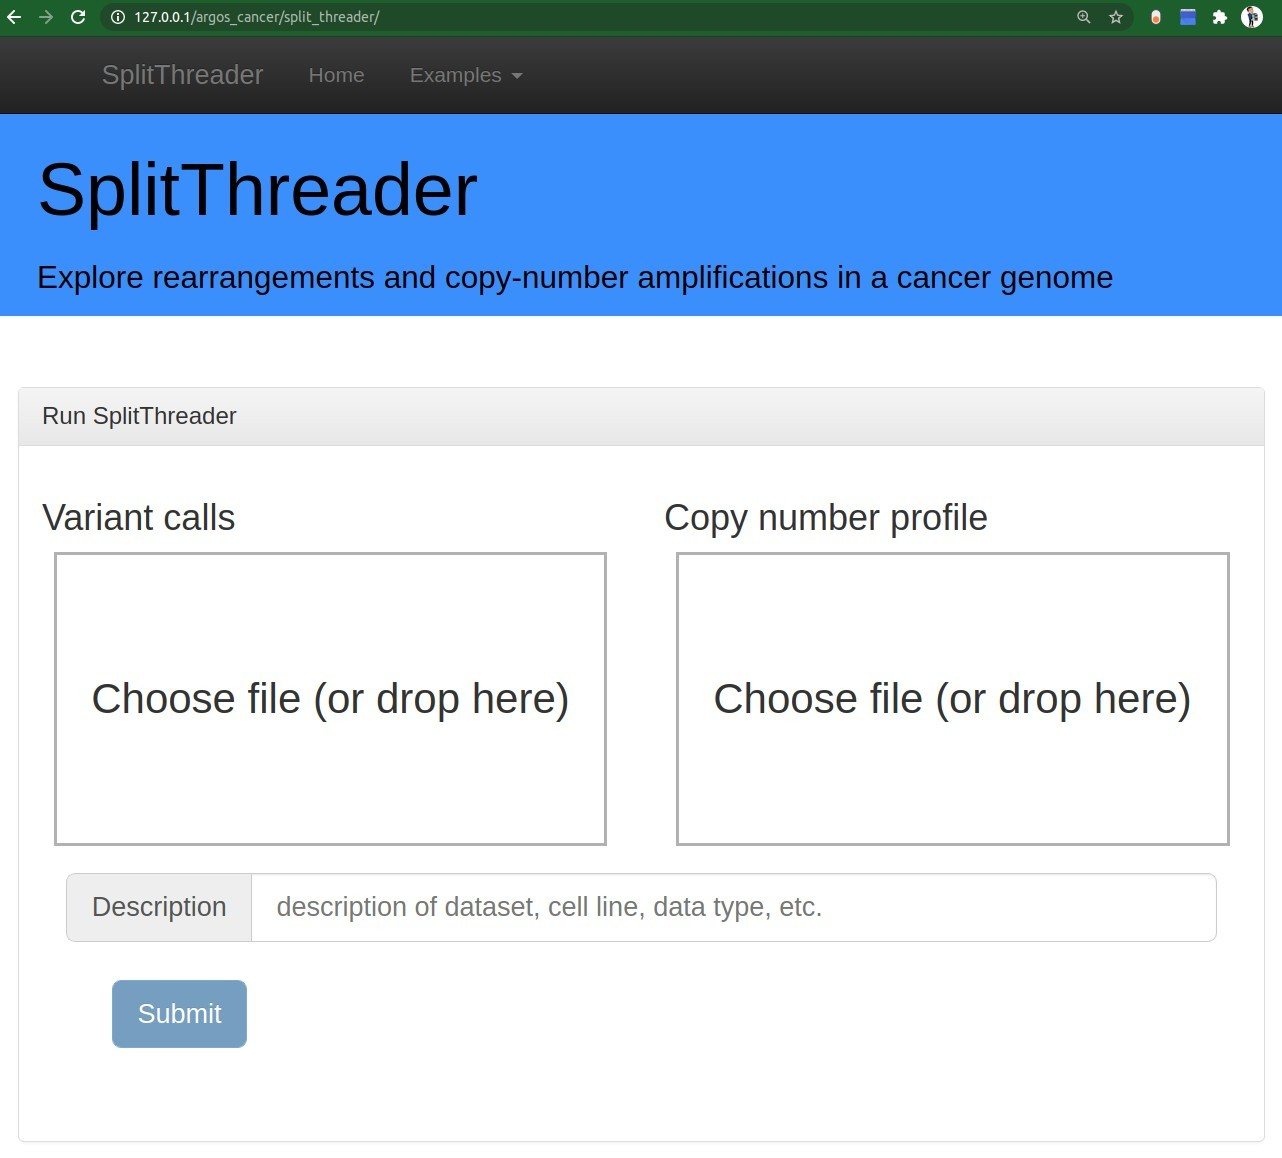
\includegraphics[width=0.6\textwidth]{img/splitthreader/split_threader_1}
	\caption{SplitThreader locally hosted. }
	\label{fig:split_threader_1}
\end{figure}

\begin{table}[H]
	\centering
	\caption{Example of a Variant Calling File (VCF). Some columns and several rows were deleted. It was built using Lumpy.}
	\label{tab:vcf}
	\begin{tabular}{ccccccccc}
		\hline
		\textbf{chrom1} & \textbf{start1}    & \textbf{stop1}     & \textbf{chrom2} & \textbf{start2}    & \textbf{stop2}     & \textbf{name} & \textbf{type} & \textbf{split} \\ \hline
		1      & 17051740  & 17051740  & 1      & 234912188 & 234912188 & 35665         & BND           & 71    \\
		1      & 47659735  & 47659735  & 8      & 105739138 & 105739138 & 573599        & BND           & 6     \\
		1      & 87069066  & 87069066  & 2      & 82854932  & 82854932  & 571553        & BND           & 6     \\
		1      & 109650635 & 109650635 & 22     & 30163373  & 30163373  & 575755        & BND           & 36    \\
		1      & 150593722 & 150593722 & 5      & 55447995  & 55447995  & 572639        & BND           & 19    \\
		1      & 153306043 & 153306043 & 16     & 76228788  & 76228788  & 575219        & BND           & 6     \\
		1      & 168186186 & 168186186 & 1      & 182274316 & 182274316 & 20968         & BND           & 11    \\
		1      & 201288206 & 201288206 & 10     & 52642286  & 52642286  & 574013        & BND           & 9     \\
		1      & 208992122 & 208992122 & 3      & 87327147  & 87327147  & 572038        & BND           & \\ 
		... \\ \hline
	\end{tabular}
\end{table}

\begin{table}[H]
	\centering
	\caption{Example of a copy number profile. It was built using Copycat.}
	\label{tab:cn}
	\begin{tabular}{cccc} 
		\hline
		\textbf{chromosome} & \textbf{start}  & \textbf{end}    & \textbf{coverage} \\ \hline
		1          & 0      & 10000  & 0        \\
		1          & 10000  & 20000  & 0.9605   \\
		1          & 20000  & 30000  & 0        \\
		1          & 30000  & 40000  & 0        \\
		1          & 40000  & 50000  & 0.0059   \\
		1          & 50000  & 60000  & 0.775    \\
		1          & 60000  & 70000  & 0.6154   \\
		1          & 100000 & 110000 & 0.3666  \\
		... \\ \hline
	\end{tabular}
\end{table}


After analysis, SplitThreader plot graphs (Figure \ref{fig:split_threader_2}). It uses a circle plot in order to show genome rearrangements. Moreover, we could see copy numbers and gene fusion for a pair of chromosomes. For instance, in Figure \ref{fig:split_threader_2}, we see chromosome 1 and chromosome 2 ( histograms), then the lines between them, represent copy regions.\\

\begin{figure}[H]
	\centering
	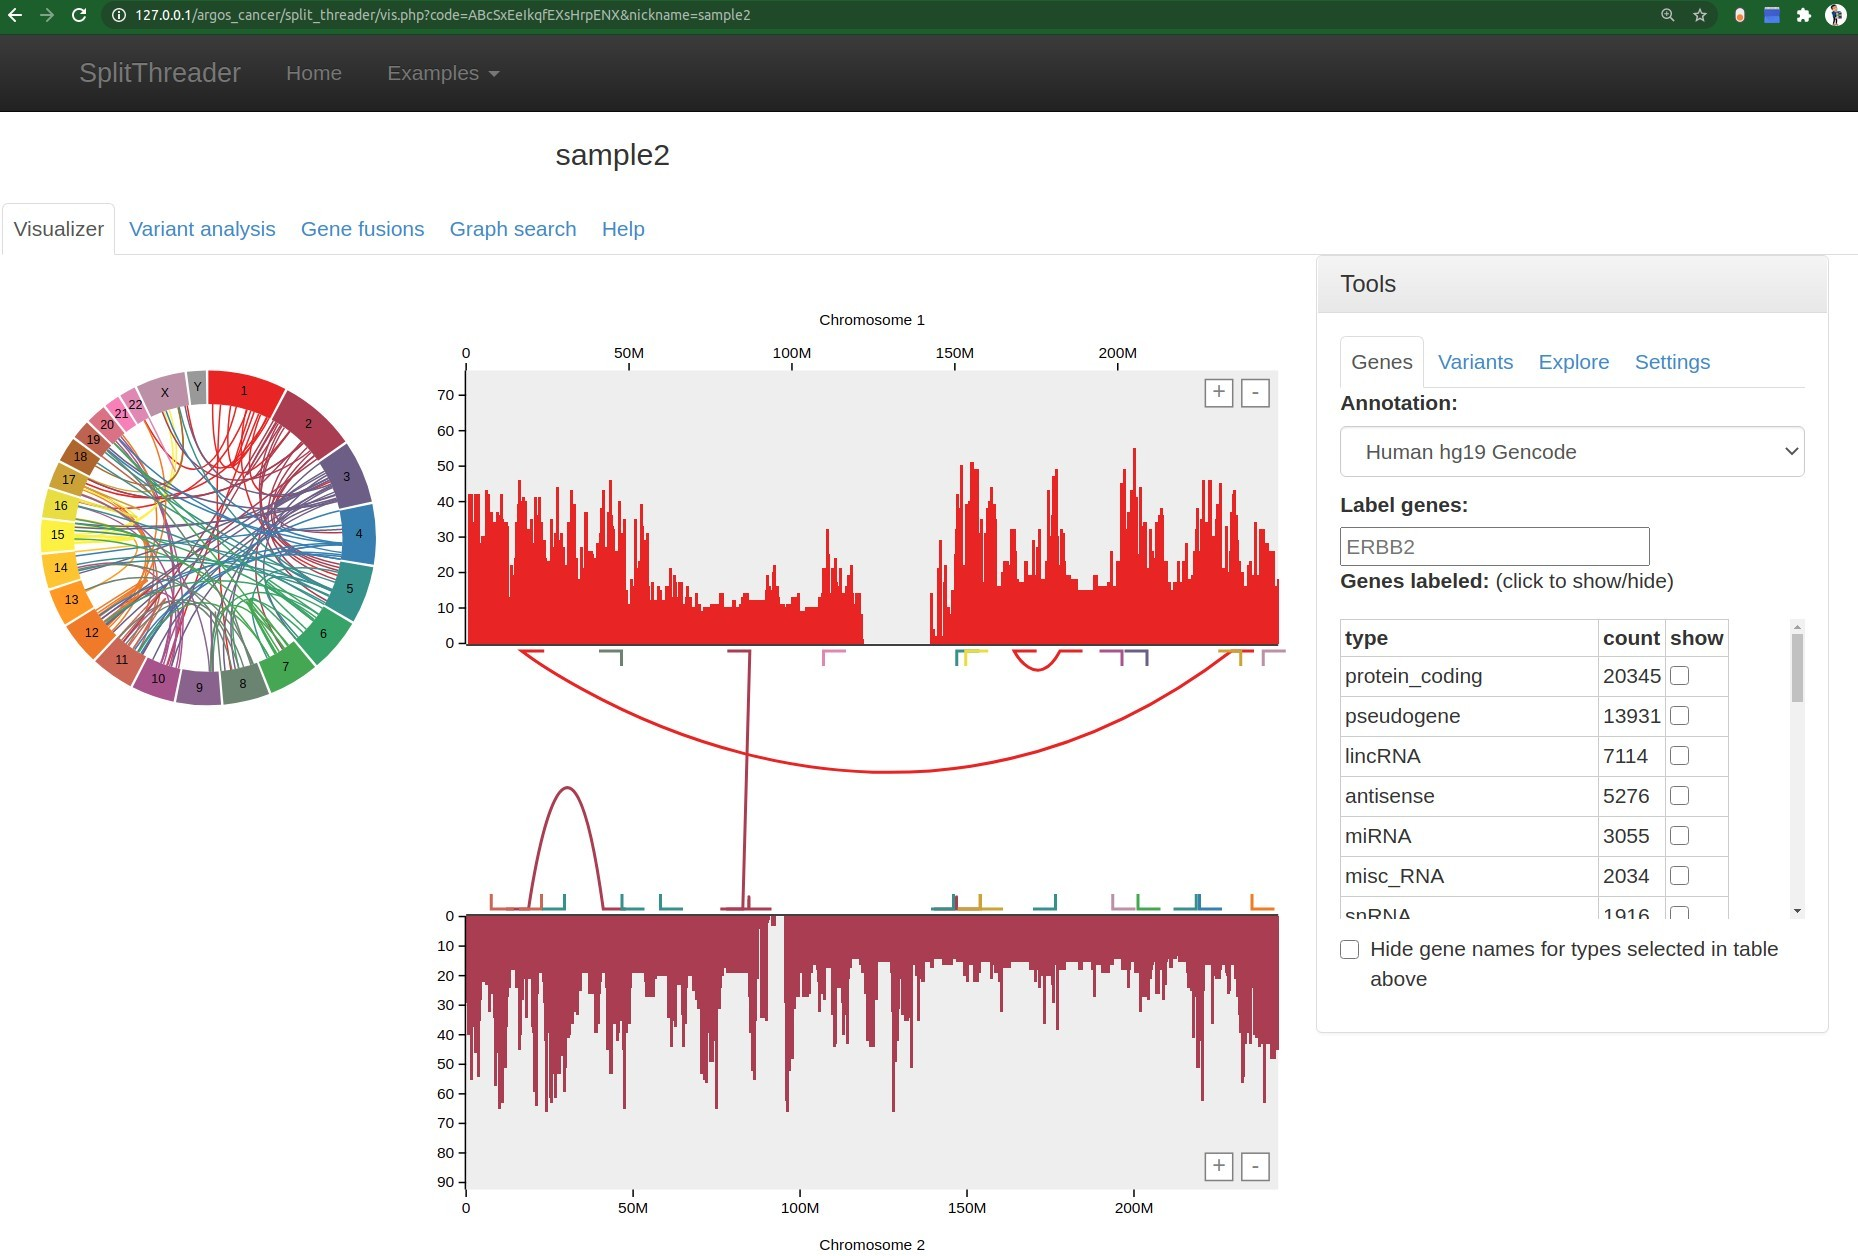
\includegraphics[width=\textwidth]{img/splitthreader/split_threader_2}
	\caption{Plots generated by SplitThreader.}
	\label{fig:split_threader_2}
\end{figure}


%%%%%%%%%%%%%%%%%%%%%%%%%%%%%%%%%%%%%%%%%%%%%%%%%%%%%%%%%%%%%%%%%%%%%%%%%%%%%%%%%%%%%
%%%%%%%%%%%%%%%%%%%%%%%%%%%%%%%%%%%%%%%%%%%%%%%%%%%%%%%%%%%%%%%%%%%%%%%%%%%%%%%%%%%%%
\section{Conclusions} \label{section:conclusions}	
%%%%%%%%%%%%%%%%%%%%%%%%%%%%%%%%%%%%%%%%%%%%%%%%%%%%%%%%%%%%%%%%%%%%%%%%%%%%%%%%%%%%%
%%%%%%%%%%%%%%%%%%%%%%%%%%%%%%%%%%%%%%%%%%%%%%%%%%%%%%%%%%%%%%%%%%%%%%%%%%%%%%%%%%%%%

In this work, we analyzed and replicated the results of SplitThreader. It is a Web tool for exploration and analysis of rearrangements in cancer genomes.\\

It is know that structural variant are key markers in cancer genomics. Most of them are related to high copy number variants and gene fusions. Nevertheless, despite the new sequencing technologies and alignment algorithm, it is difficult to detect this variants. \\

Visualization is a emerging area that can be applied in Bioinformatics, it is used in Proteomics, Genomics, Metagenomics and Cancer genomics. Moreover, several tools have emerged like SplitThreader and MoMI-G to help the analysis and visualization of structural variants and its relation in cancer genomes.\\

SplitThreader have a simple architecture but it is robust for genome analysis. It basically uses PHP to perform API Restfull services and Javascript to plot the graphs. Additionally, it uses R and Python scripts for processing the data.\\

Finally, SplitThreader uses a breath-first search algorithm in order to detect gene fusions, then it plots copy number variants and gene fusions graphically. Nevertheless, the results of SpliThreader depends on  Lumpy and Sniffles.   

% ---- Bibliography ----
%\clearpage
\bibliographystyle{unsrt}
\bibliography{bibliography}

\end{document}
